\documentclass[dvipdfmx]{jsarticle}
\usepackage[dvipdfmx]{graphicx}
\usepackage{multicol}
\usepackage{amsthm}
\usepackage[]{multicol}
\usepackage{amsmath}
\usepackage{fancybox}
\usepackage{ascmac}
\usepackage{mathrsfs}
\usepackage{amsfonts}
\usepackage{amssymb}
\usepackage{tikz}
\usepackage{wrapfig}
\usepackage{latexsym}
\usepackage{MnSymbol}
\graphicspath{{../AMC002-picture/}}
\usetikzlibrary{cd}
\newtheorem*{answer*}{解答}
\newtheorem{prob}{}[]
\newtheorem{definition}[prob]{定義}
\newtheorem{dfn}[prob]{定義}
\newtheorem{theorem}[prob]{定理}
\newtheorem*{lemma*}{補題}
\newtheorem{answer}{解答}
\newtheorem*{proof*}{証明}
\begin{document}


\hskip1zw {\Large Asahi\ Math Contest 002 解答} 
\hskip1zw R3.9.11 第$74$回朝日祭\\  % \hskipは水平方向にスペースを作ります
\rightline {岡山朝日数学同好会}\\
\underline{\hskip2zw年 \hskip2zw 組 \hskip2zw 番\hskip1zw 氏名 \hskip30ex} 

%大問1
\begin{screen}
  \begin{prob}
    $1$本の道路があり,図$1$のように枝分かれしている.
    枝分かれした道路の先には必ず労働者の家がある.
    いま,この道路のどこかにバス停をひとつ作ることを考える.
    各労働者の家からバス停までの移動距離の合計がもっとも短くなるようにするにはどこにバス停を作ればよいか.
  \end{prob} 
  \end{screen}
  \begin{figure}[h]
    \centering
    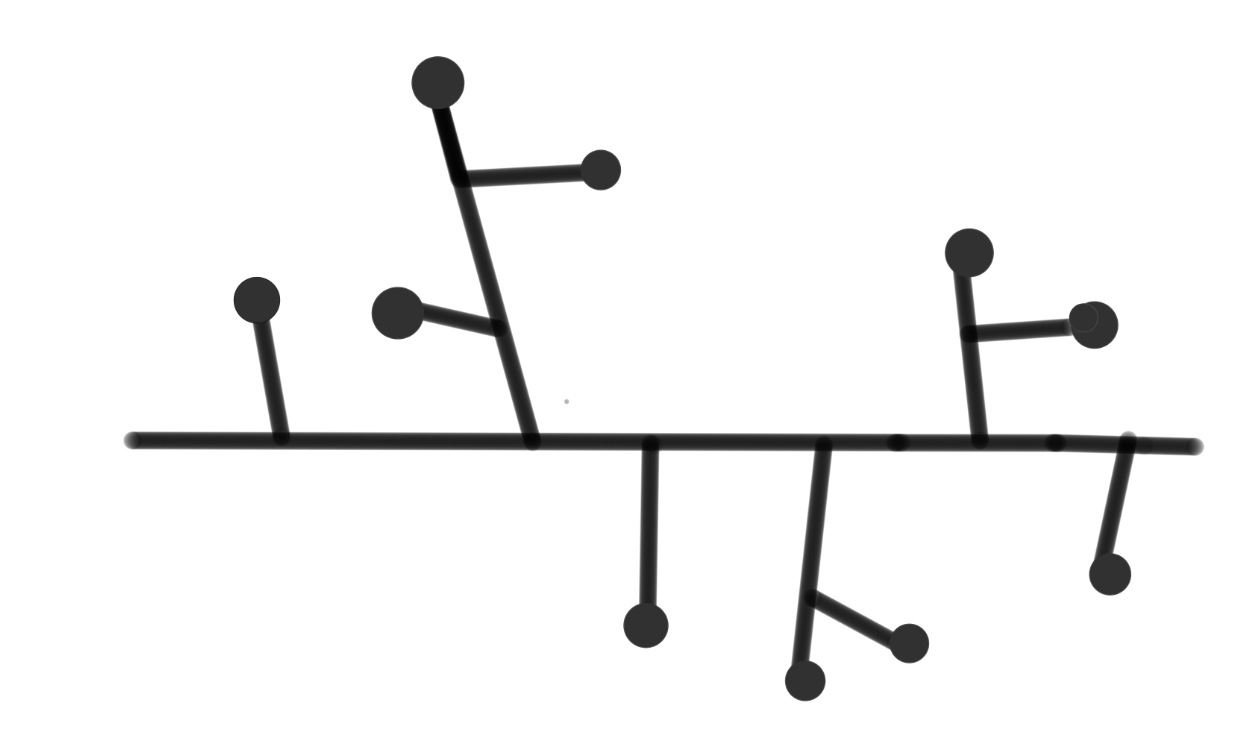
\includegraphics[width=14cm]{AMC002-picture/mathtest3.png}
    \caption {}\label{ex3}
  \end{figure}
  \begin{answer*}
    答えは左から$3$番目と$4$番目の付け根を含む$2$地点のいずれかの地点である.\\
    もし,それ以外の場所に存在したとき,バス停によって分けられた家の集合の要素数に差により距離の偏りが生じ,距離が増加するため不適合である.
  \end{answer*}
\newpage
%大問2
\begin{screen}
  \begin{prob}
    数列$\{a_{n}\}$が$a_{1}=3,(2n+1)a_{n+1}=2na_{n}+1$を満たすとき,$a_{n}$を$n$を用いて表せ.
  \end{prob}
\end{screen}
\begin{answer*}
  変形すると,
  \begin{align*}
    (2n+1)(a_{n+1}-1) &= 2n(a_{n}-1)
  \end{align*}
  $n \geq 2$において,
  \begin{align*}
    a_{n}-1=\frac{2n-2}{2n-1}(a_{n-1}-1)
  \end{align*}
  これを繰り返して,
  \begin{align*}
    a_{n}-1&=\frac{2n-2}{2n-1}\times \frac{2n-4}{2n-3}\times \cdots \times (a_{1}-1)
    =\frac{2^{n-1}(n-1)!}{(2n!)}\times 2
    =\frac{4^nn!(n-1)!}{(2n)!}
  \end{align*}
  \begin{align*}
    a_{n}=\frac{4^nn!(n-1!)}{(2n)!}+1
  \end{align*}
  で,これは$n=1$ でもこれは成立するため
  \begin{align*}
    a_{n}=\frac{4^nn!(n-1!)}{(2n)!}+1
  \end{align*}
  が求める答えである.

\end{answer*}

%大問3
\begin{screen}
  \begin{prob}
    $O$を原点とする$xyz$空間座標系において,$xy$平面上の点ではない$2$点$A,B$からそれぞれ$xy$平面へ下ろした垂線の足を$P,Q$とおく.
    $\angle AOP=\alpha ,\angle BOQ=\beta,\angle POQ=\gamma$とするとき,
    $\cos \angle AOB$を$\alpha,\beta,\gamma$を用いて表せ.  
  \end{prob}
  \end{screen}
\begin{answer*}
    余弦定理より,
    \begin{align*}
      \operatorname{AB}^2=\operatorname{OA}^2+\operatorname{OB}^2-2\operatorname{OA}\cdot\operatorname{OB}\cdot\cos \angle\operatorname{AOB}\tag{1}
    \end{align*}
    点$\operatorname{A},\ \operatorname{B}$から$z$軸への垂線の足をそれぞれ$\operatorname{R},\ \operatorname{S}$とすると
    \begin{align*}
      \operatorname{AB}^2=\operatorname{AR}^2+\operatorname{BR}^2-2\operatorname{AR}\cdot\operatorname{BR}\cdot\cos \angle\operatorname{ARB}\tag{2}
    \end{align*}
    ここで$\overrightarrow{\operatorname{RA}} $と同じ向きの単位ベクトルを$\overrightarrow{e}$とおくと,$\overrightarrow{e}\bot \overrightarrow{RS} $より,
    \begin{align*}
      \overrightarrow{e}\cdot\overrightarrow{\operatorname{RB}}
      &= \overrightarrow{e}\cdot \left(\overrightarrow{\operatorname{RS}}+ \operatorname{SB}\right)\\
      &= \operatorname{SB}\cos \gamma \\
      \therefore \operatorname{RB}\cos \angle ARB&=\operatorname{SB}\cos \gamma
    \end{align*}
    三平方の定理より,$\operatorname{RB}^2=\operatorname{BS}^2+\operatorname{RS}^2$であるから,
    \begin{align*}
      (1)
      &\Longleftrightarrow \operatorname{AB}^2=\operatorname{AR}^2+(\operatorname{BS}^2+\operatorname{RS}^2)-2\operatorname{AR}\cdot\operatorname{BS}\cos\gamma\\
      &\Longleftrightarrow \operatorname{OB}^2+\operatorname{OB}^2-2\cdot\operatorname{OA}\cdot\operatorname{OB}(\sin\alpha\sin\beta+\cos\alpha\cos\beta\cos\gamma)\tag{3}
    \end{align*}
    $(1),\ (3)$を比較して,
    \begin{align*}
      \cos\angle\operatorname{AOB}=\sin\alpha\sin\beta+\cos\alpha\cos\beta\cos\gamma
    \end{align*}
    \rightline{$\Large{\Box} $}
\end{answer*}
  \newpage
  
\newpage

%大問4
\begin{screen}
  \begin{prob}
    $n$を$3$以上の整数とする.$1$辺の長さを$1$とする正$2n$角形の最も短い対角線の長さを$l_{n}$,最も長い対角線の長さを$L_{n}$とする.このとき,以下の級数の収束・発散を判定せよ.また,収束するならばその和を求めよ.
  \begin{align*}
    \sum_{n=3}^{\infty}{\frac{1}{l_{n}\cdot L_{n}}}
  \end{align*} 
  \end{prob}
\end{screen}
\begin{answer}
  \begin{figure}[h]
    \centering
    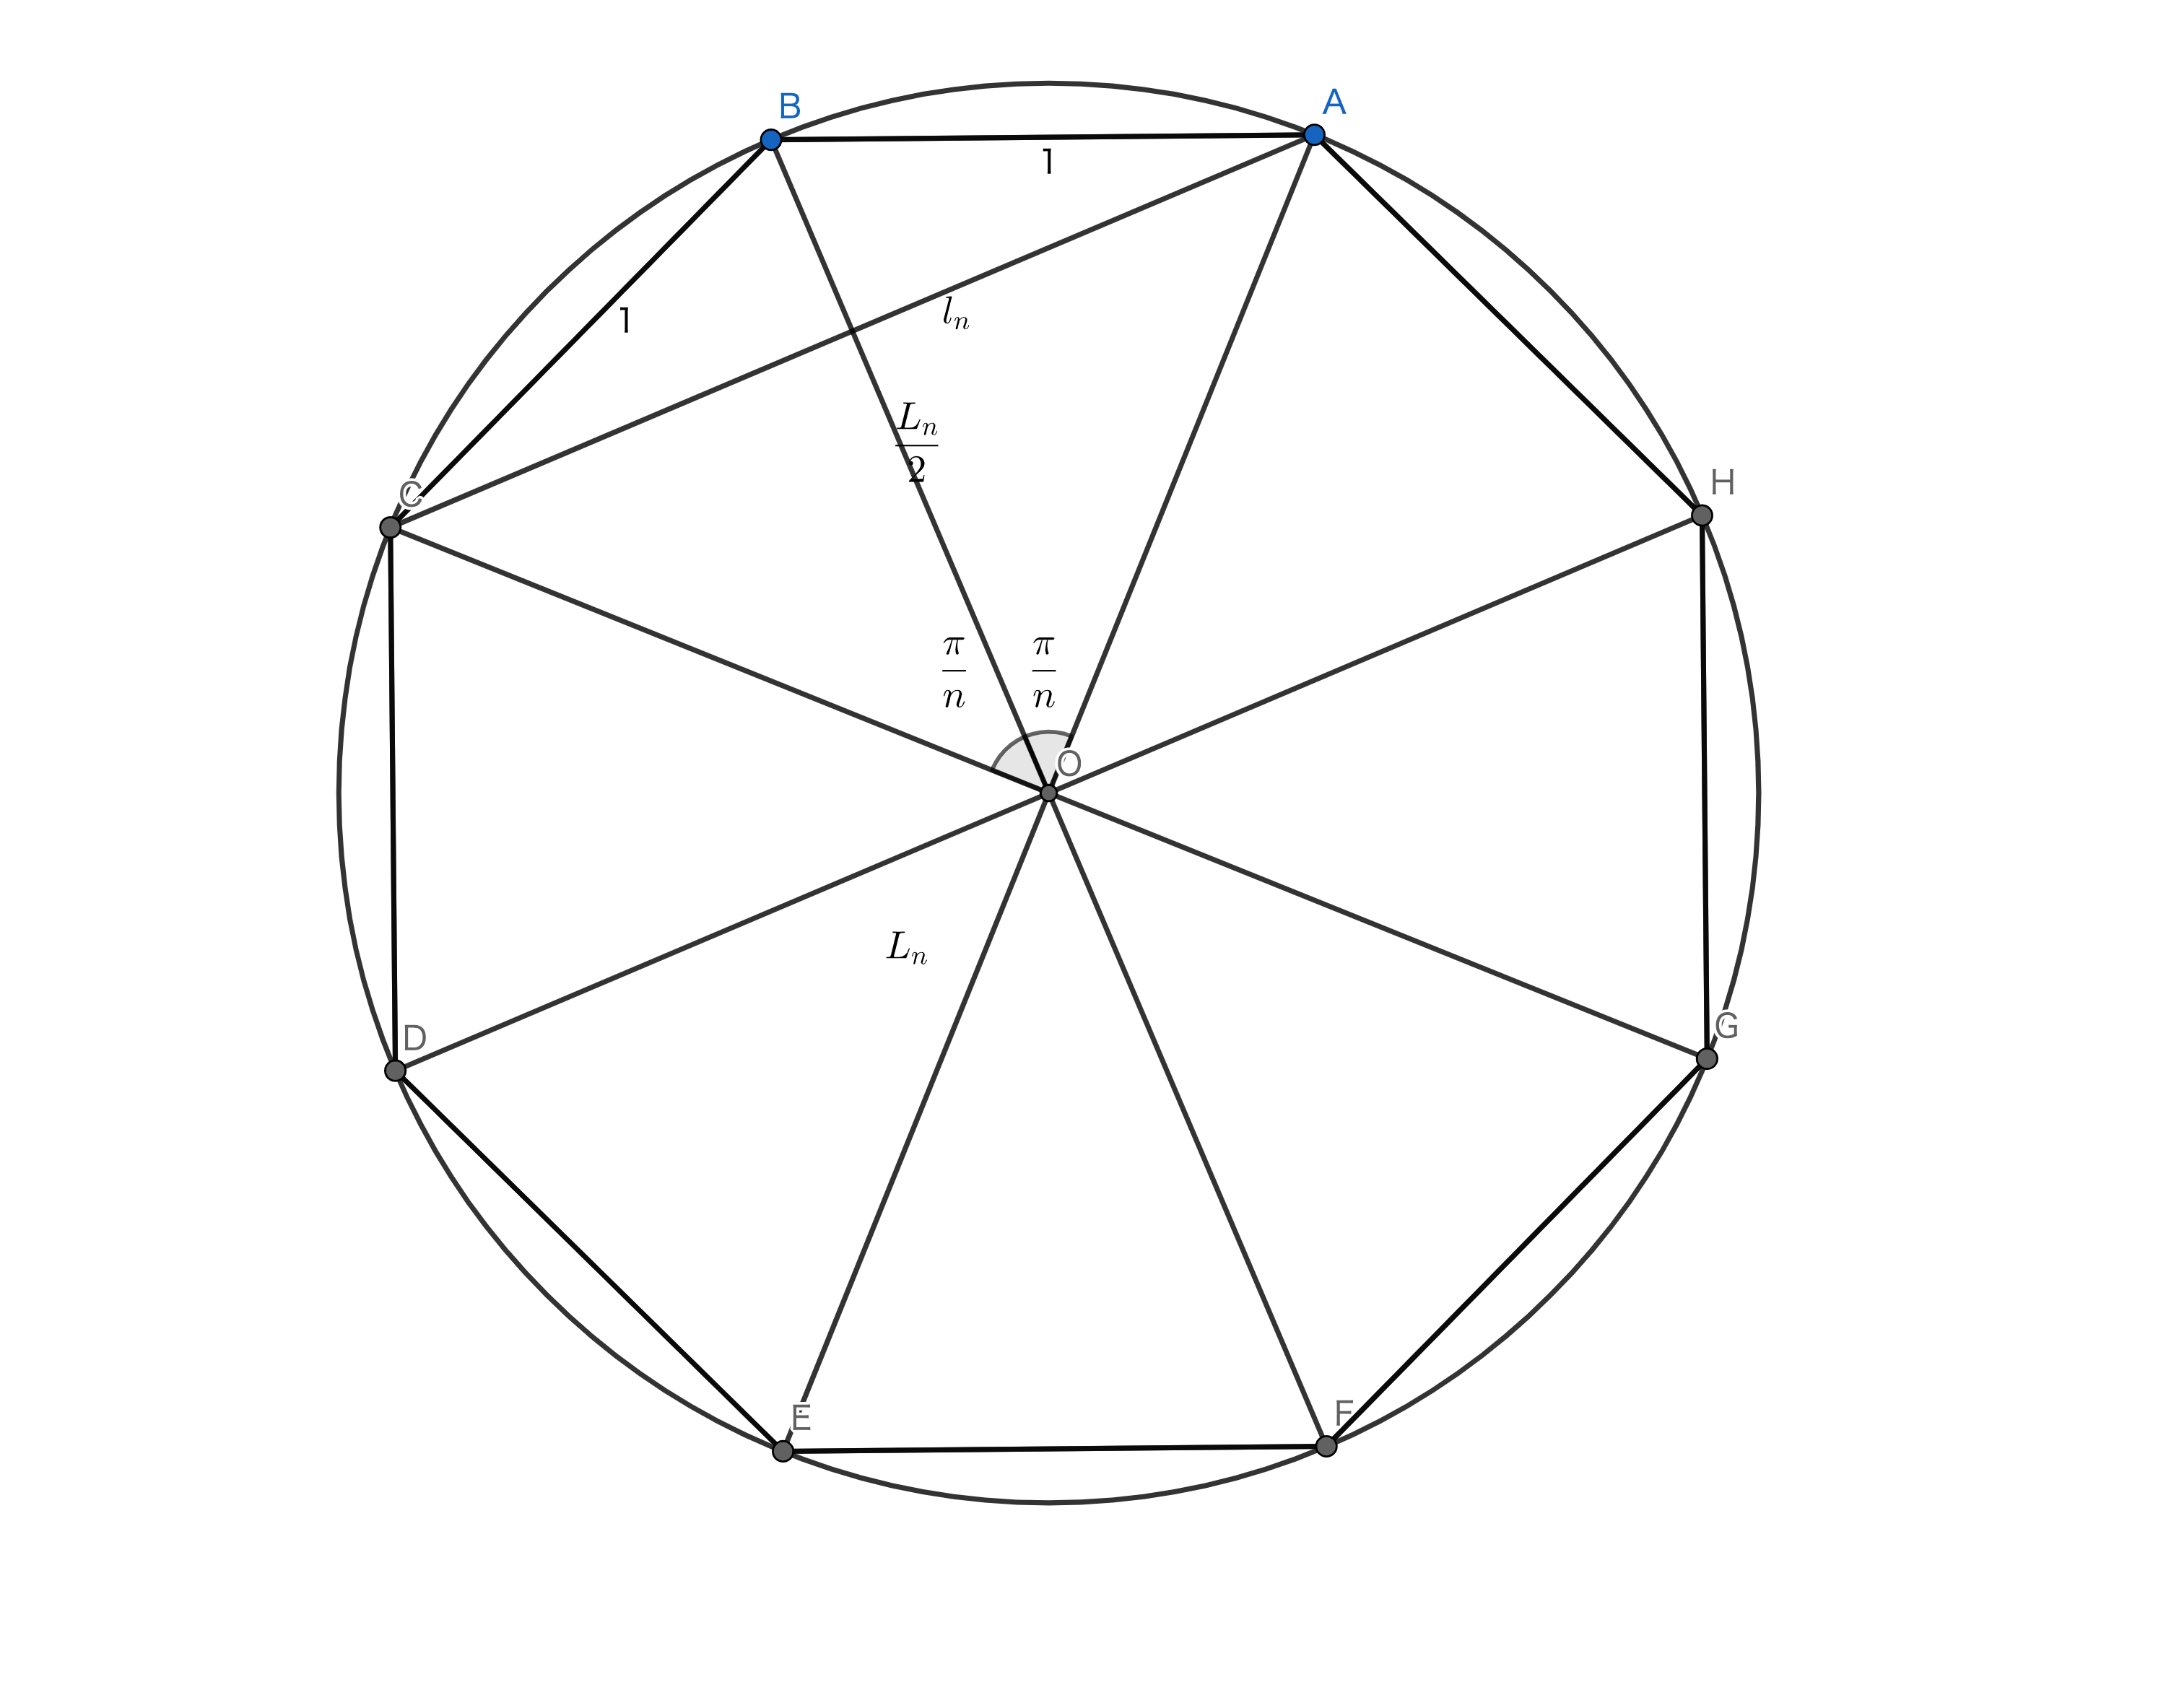
\includegraphics[width=7cm]{AMC002-picture/mathtest1.png}
    \caption {}\label{ex1}
  \end{figure}
    $\frac{\pi}{2n}=\theta $とおく.
    $L_{n}=1/\sin \theta$,$l_{n}=2\cos \theta$より,
    
  \begin{align*}
    \sum_{n=3}^{\infty}{\frac{1}{l_{n}\cdot L_{n}}}=\sum_{n=3}^{\infty}\frac{\tan \theta}{2}
  \end{align*}
    $0<\theta<\frac{\pi}{2}$において,$1<(\tan \theta)'=\frac{1}{\cos ^{2}\theta}$
    $\theta '=1$より,$\tan \theta >\theta$であるから,
  \begin{align*}
    \sum_{n=3}^{\infty}\frac{\tan \theta}{2}>\frac{1}{2}\sum_{n=3}^{\infty}\frac{1}{n}=\infty
  \end{align*}
    よって,求値式は発散する.\\
    \rightline{$\Box $}
\end{answer}
\begin{answer}
  トレミーの定理より,
  \begin{align*}
    l_{n}L_{n}=2\sqrt{L^{2}_{n}-1}
  \end{align*}
  $L_{n}\leq $正多角形の周の長さの半分の長さ$n$より,
  \begin{align*}
    \sum_{n=3}^{\infty}{\frac{1}{l_{n}\cdot L_{n}}}=\sum_{n=3}^{\infty}{\frac{1}{2\sqrt{L^{2}_{n}-1}}}
    \geq \sum_{n=3}^{\infty}\frac{1}{2n}=\infty
  \end{align*}
  よって,求値式は発散する.\\
  \rightline{$\Box $}
\end{answer}
 

%大問5
\begin{screen}
\begin{prob}
   $p$を素数とする.このとき,
\begin{align*}
  \sum_{n=1}^{p-1}\binom{p-1}{n}\frac{1}{n^{2p}} 
\end{align*}
  を既約分数で表したとき,分子は$p$で最大何回割り切れるか. 
\end{prob}
\end{screen}
\begin{answer*}
  $n!$と$p$は互いに素なので,
  \begin{align*}
    (p-1)(p-2)\cdots (p-n)\equiv (-1)^n\cdot n! \pmod{p}
  \end{align*}
  よって$\binom{p-1}{n}\equiv (-1)^n\pmod{p}$であるから,示すべきは
  \begin{align*}
    \sum_{n=1}^{p-1}(-1)^n\frac{1}{n^{2p}} 
  \end{align*}
  の分子が$p^2$で割り切れることである.\\
  また,フェルマーの小定理より,
  \begin{align*}
    \sum_{n=1}^{p-1}(-1)^n\frac{1}{n^{2}}
    \equiv \sum_{n=1}^{p-1}(-1)^nn^2 
    \equiv \sum_{n=1}^{\frac{p-1}{2}}\left(4n+1\right)=p\frac{p-1}{2}
    \pmod p 
  \end{align*}
  よって,分子は$p$で$1$回割り切れる.
  \rightline{$\Large{\Box} $}
\end{answer*}

%大問6
\begin{screen}
  \begin{prob}
    次の値を求めよ.
    \begin{align*}
      \int_{0}^{\frac{1}{\sqrt[3]{2} }}  \frac{\,dx }{\sqrt[3]{1-x^3}}
   \end{align*}
  \end{prob}
\end{screen}
\begin{answer*}
  $x=\frac{t}{\sqrt[3]{t^3+1}}$,$t=\frac{\sqrt{3}}{2}\tan \theta+\frac{1}{2}$とおく.このとき,
  \begin{align*}
    \int_{0}^{\frac{1}{\sqrt[3]{2} }} \frac{\,dx }{\sqrt[3]{1-x^3}} 
    &=\int_{0}^{1}\frac{\,dt}{t^3+1}  \,dx \\
    &=\frac{1}{3}\int_{0}^{1}\frac{\,dt}{t+1}  \,dt -\frac{1}{6}\int_{0}^{1}  \frac{2t-1}{t^2-t+1}\,dt +\frac{1}{2}\int_{0}^{1}  \frac{\,dt }{t^2-t+1}\\   
    &=\frac{1}{3}\left[\log {\left\lvert t+1\right\rvert }\right]_{0}^{1} -\frac{1}{6}\left[\log \left(t^2-t+1\right)\right]_{0}^{1} + \frac{1}{2}\int_{0}^{1}  \frac{\,dt }{\left(t-\frac{1}{2}\right)^2+\frac{3}{4}}\\
    &=\frac{1}{3}\log {2}+\frac{\sqrt{3}}{3}\int_{-\frac{\pi}{6}}^{\frac{\pi}{6}}  \,d\theta \\
    &=\frac{1}{3}\log {2}+\frac{\sqrt{3}}{6}\pi
  \end{align*}
  \rightline{$\Box $}
\end{answer*}
\newpage

%大問7
\begin{screen}
  \begin{prob}
    $p$を素数,$n,k\in \mathbb{N}$,$m$を$p\nmid m$を満たす自然数とする.このとき,
\begin{align*}
  \sum_{i=0}^{n}(-1)^i\binom{n}{i}\binom{p^km+n-i}{p^k-i}
\end{align*}
は$p$で割り切れるか.
  \end{prob}
\end{screen}
\begin{answer*}
  $X:=\{x_{1},\cdots,x_{n}\}$を$n$個の青いボールからなる集合.$Y$を$p^km$個の赤いボールからなる集合として,
  赤いボールのみの要素数$p^k$個$(Z=X\cup Yの)$の部分集合の総数を数えることと同値である.よって包除原理より,
  \begin{align*}
  \sum_{i=0}^{n}(-1)^i\binom{n}{i}\binom{p^km+n-i}{p^k-i}=\binom{p^km}{p^k} 
  \end{align*}
  となる.
  \begin{align*}
    \binom{p^km}{p^k}=\frac{p^km(p^km-1)\cdots(p^km-p^k+1)}{p^k(p^k-1)\cdots 1}
  \end{align*}
  分子の約数$p$は$p^km-i$あるいは$p^k-i$の約数からなる.$\gcd(m,p)=1$で$1\leq i<p^k$
  のとき,$p^t\mid p^km-i$となる必要十分条件は$p^t\mid i$となることである.したがって,
  $p^km-i$を割り切る$p$の最大の冪は$p^k-i$を割り切る$p$の最高冪と等しい.よって上段の全ての約数$p$は下段の約数$p$により割り切られる.
  よって二項係数は約数$p$を持たない.
\end{answer*}


%大問8
\begin{screen}
  \begin{prob}
    $xyz$空間座標系において,点$O(0,0,0)$,$P(a,b,c)$を通る直線を軸とする半径$r$の円柱面の方程式を求めよ.
  \end{prob}
\end{screen}
\begin{answer*}
  円柱面を集合$\Omega $とおくと,
  \begin{align}
    Q(x,\ y,\ z)\in \Omega \Longleftrightarrow  点Qと軸との距離がr.
  \end{align}
  $\overrightarrow{\operatorname{OP}} $と$\overrightarrow{\operatorname{OQ}}$による平行四辺形の面積を$S$とおくと,
  \begin{align*}
    (1)
    &\Longleftrightarrow S=r\sqrt{a^2+b^2+c^2}\\
    &\Longleftrightarrow \left\lvert \overrightarrow{\operatorname{OP}}\times \overrightarrow{\operatorname{OQ}}\right\rvert =r\sqrt{a^2+b^2+c^2}\\
    &\Longleftrightarrow\left\lvert 
    \begin{pmatrix}
      ay-bx\\
      bz-cy\\
      cx-az
    \end{pmatrix}
    \right\rvert =r\sqrt{a^2+b^2+c^2}\\
    &\Longleftrightarrow \sqrt{(ay-bx)^2+(bz-cy)^2+(cx-az)^2}=r\sqrt{a^2+b^2+c^2}\\
    &\Longleftrightarrow (ay-bx)^2+(bz-cy)^2+(cx-az)^2=r^2(a^2+b^2+c^2)\\
  \end{align*}
  \rightline{$\Box $}
\end{answer*}
\newpage
%大問9
\begin{screen}
  \begin{prob}
    空間上に正四面体$OXYZ$がある.点$P$が準格子点であるとは,ある整数$a,b,c$が存在し,
  \begin{align*}
    \overrightarrow{OP}=a\overrightarrow{OX}+b\overrightarrow{OY}+c\overrightarrow{OZ}  
  \end{align*}
  を満たすことをいう.このとき,正多面体に関する次の条件を満たすものを全て挙げよ.
  \begin{align*}
    (*)準格子点を結ぶことで作れない.
  \end{align*}  
  \end{prob} 
\end{screen}
\begin{answer*}
\end{answer*}
\begin{figure}[h]
  \centering
  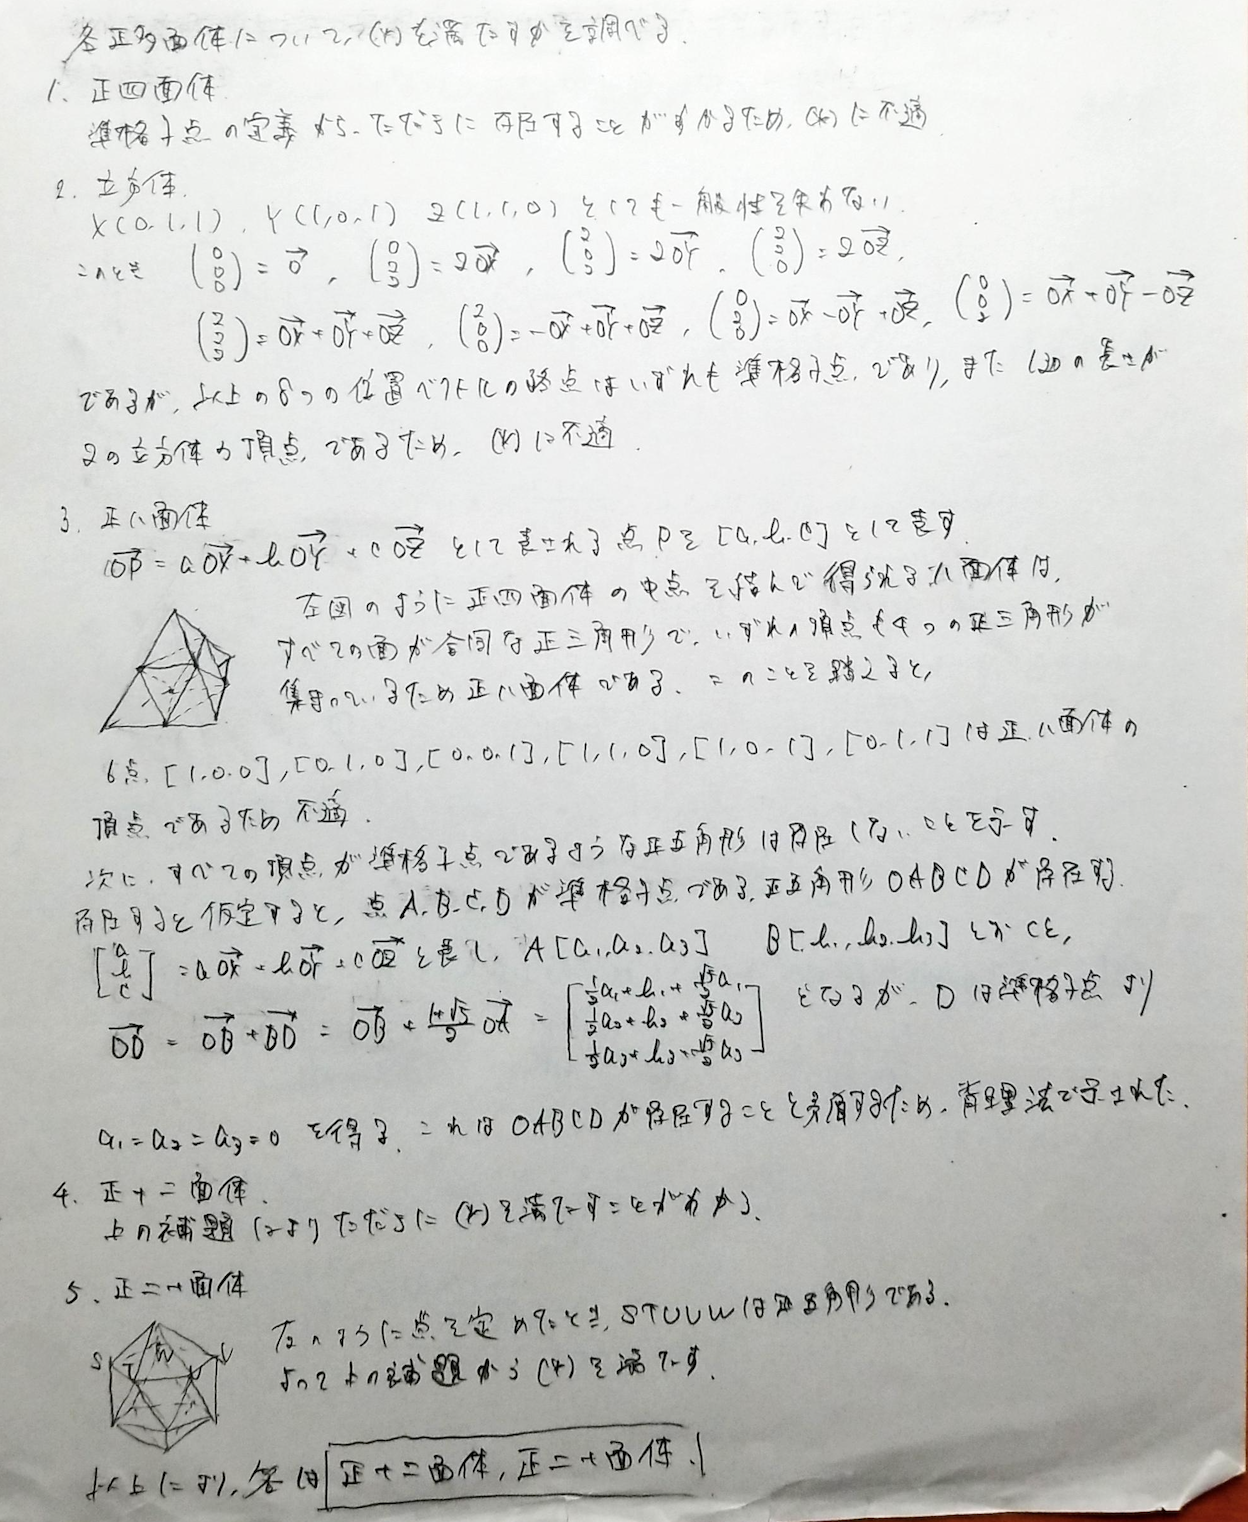
\includegraphics[width=14cm]{AMC002-picture/mathtest4.png}
\end{figure}
\newpage

%大問10
\begin{screen}
  \begin{prob}
    領域$0\leq x \leq \frac{\pi}{2}$において,曲線$y=-3\cos x+2$と$2$直線$x=1$,$y=-1$で囲まれた図形の面積を$S_{1}$,
    曲線$y=-4\cos x+2$と$2$直線$x=1$,$y=-2$で囲まれた図形の面積を$S_{2}$,$2$曲線$y=-2\cos x+2$,$y=-4\cos x+2$と$y$軸で囲まれる面積から
    $0\leq x \leq 1$,$-2\leq y\leq 0$の部分を除いた図形の面積を$S_{3}$とする.このとき,$S_{1}$:$\left(S_{2}+S_{3}\right)$を最も簡単な整数比で表せ.
  \end{prob}

\end{screen}
\begin{answer*}
  \begin{figure}[h]
    \centering
    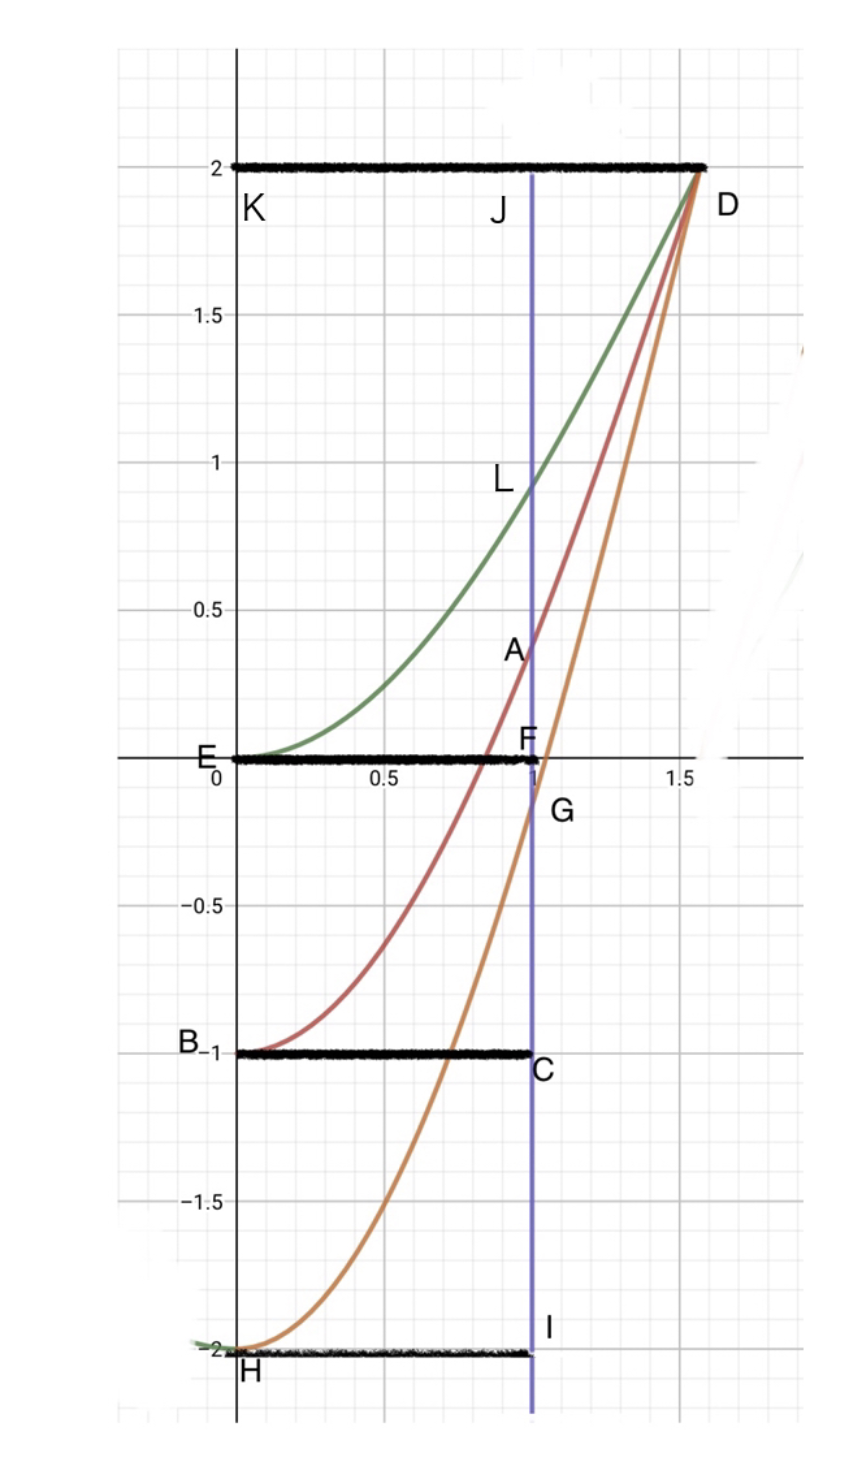
\includegraphics[width=5.5cm]{AMC002-picture/mathtest2.png}
    \caption {}\label{ex2}
  \end{figure}
  まず,
  \begin{align*}
    図形\operatorname{ABC}+図形\operatorname{ABKJ}&=3\\
    図形\operatorname{ABKJ}+図形\operatorname{AJD}&=3\int_{0}^{\frac{\pi}{2}}  \cos x\,dx =2\left[\sin x\right]^{\frac{\pi}{2}}_{0}=3 
  \end{align*}
  であるから,図形$\operatorname{ABC}=$図形$\operatorname{AJD}=S_{1}$.\\
  同様に,
  \begin{align*}
    図形\operatorname{FEL}&=図形\operatorname{DJL}=\frac{2}{3}S_{1}\\
    S_{2}=図形\operatorname{GHI}&=図形\operatorname{DGJ}=\frac{4}{3}S_{1}\\
    図形\operatorname{DGL}&=図形\operatorname{DGJ}-図形\operatorname{DJL}=\frac{4}{2}S_{1}-\frac{2}{3}S_{1}=\frac{2}{3}S_{1}\\
    S_{2}+S_{3}=図形\operatorname{FEL}&+図形\operatorname{GHI}+図形\operatorname{DGL}=\frac{2}{3}S_{1}+\frac{4}{3}S_{1}+\frac{2}{3}S_{1}=\frac{8}{3}S_{1}
  \end{align*}
  よって求めるのは$S_{1}$:$\left(S_{2}+S_{3}\right)=3$:$8$\ .\\
  \rightline{$\Box $}
\end{answer*} 
\end{document}


